\documentclass{article}
\usepackage{microtype}
\usepackage{graphicx}
\usepackage{subcaption}
\usepackage{booktabs} % for professional tables
\usepackage{hyperref}
\usepackage{libertine}
\usepackage{graphicx}
\usepackage[svgnames]{xcolor}
\usepackage{tikz}
\usepackage{placeins}
\usepackage{dsfont}
\usepackage{natbib}

\newcommand{\set}[1]{\lbrace#1\rbrace}
\newcommand{\e}{\mathrm{e}}

\makeatletter
\setlength{\@fptop}{0pt}
\makeatother

\renewcommand{\topfraction}{0.9}      % max fraction of floats at top
\renewcommand{\dbltopfraction}{0.9}   % for two-column floats
\setcounter{topnumber}{2}             % max floats at top
\setcounter{dbltopnumber}{2}          % for two-column


\newcommand{\theHalgorithm}{\arabic{algorithm}}

\usepackage{icml2026}
\usepackage{amsmath}
\usepackage{amssymb}
\usepackage{mathtools}
\usepackage{amsthm}
\usepackage[capitalize,noabbrev]{cleveref}


\theoremstyle{plain}
\newtheorem{theorem}{Theorem}[section]
\newtheorem{proposition}[theorem]{Proposition}
\newtheorem{lemma}[theorem]{Lemma}
\newtheorem{corollary}[theorem]{Corollary}
\theoremstyle{definition}
\newtheorem{definition}[theorem]{Definition}
\newtheorem{assumption}[theorem]{Assumption}
\theoremstyle{remark}
\newtheorem{remark}[theorem]{Remark}

\setlength{\marginparwidth}{1.6cm}

\icmltitlerunning{MetaOthello: A Controlled Study of Multiple World Models in Transformers}

\begin{document}

\twocolumn[
  \icmltitle{MetaOthello: A Controlled Study of Multiple World Models in Transformers}

  \icmlsetsymbol{equal}{*}

  \begin{icmlauthorlist}\icmlauthor{Anonymous}{anon}\end{icmlauthorlist}

  \icmlaffiliation{anon}{Anonymous Institution}
  
  

  \icmlcorrespondingauthor{Anonymous}{anonymous@anonymous.invalid}


  \icmlkeywords{mechanistic interpretability, world models, multi-task learning, representation geometry, othello-gpt, linear probes, function vectors}

  \vskip 0.3in
]

\printAffiliationsAndNotice{\icmlEqualContribution}

\begin{abstract}
Foundation models must handle multiple generative processes, yet mechanistic interpretability largely studies capabilities in isolation; it remains unclear how a single transformer organizes multiple, potentially conflicting ``world models''. Previous experiments on Othello playing neural-networks test world-model learning but focus on a single game with a single set of rules. We introduce \textit{MetaOthello}, a controlled suite of Othello variants with shared syntax but different rules or tokenizations, and train small GPTs on mixed-variant data to study how multiple world models are organized in a shared representation space. We find that transformers trained on mixed-game data do not partition their capacity into isolated sub-models; instead, they converge on a mostly shared board-state representation that transfers causally across variants. Linear probes trained on one variant can intervene on another's internal state with effectiveness approaching that of matched probes. For isomorphic games with token remapping, representations are equivalent up to a single orthogonal rotation that generalizes across layers. When rules partially overlap, early layers maintain game-agnostic representations while a middle layer identifies game identity, and later layers specialize. \textit{MetaOthello} offers a path toward understanding not just whether transformers learn world models, but how they organize many at once.

\end{abstract}

\section{Introduction}

\begin{figure*}
    \centering
    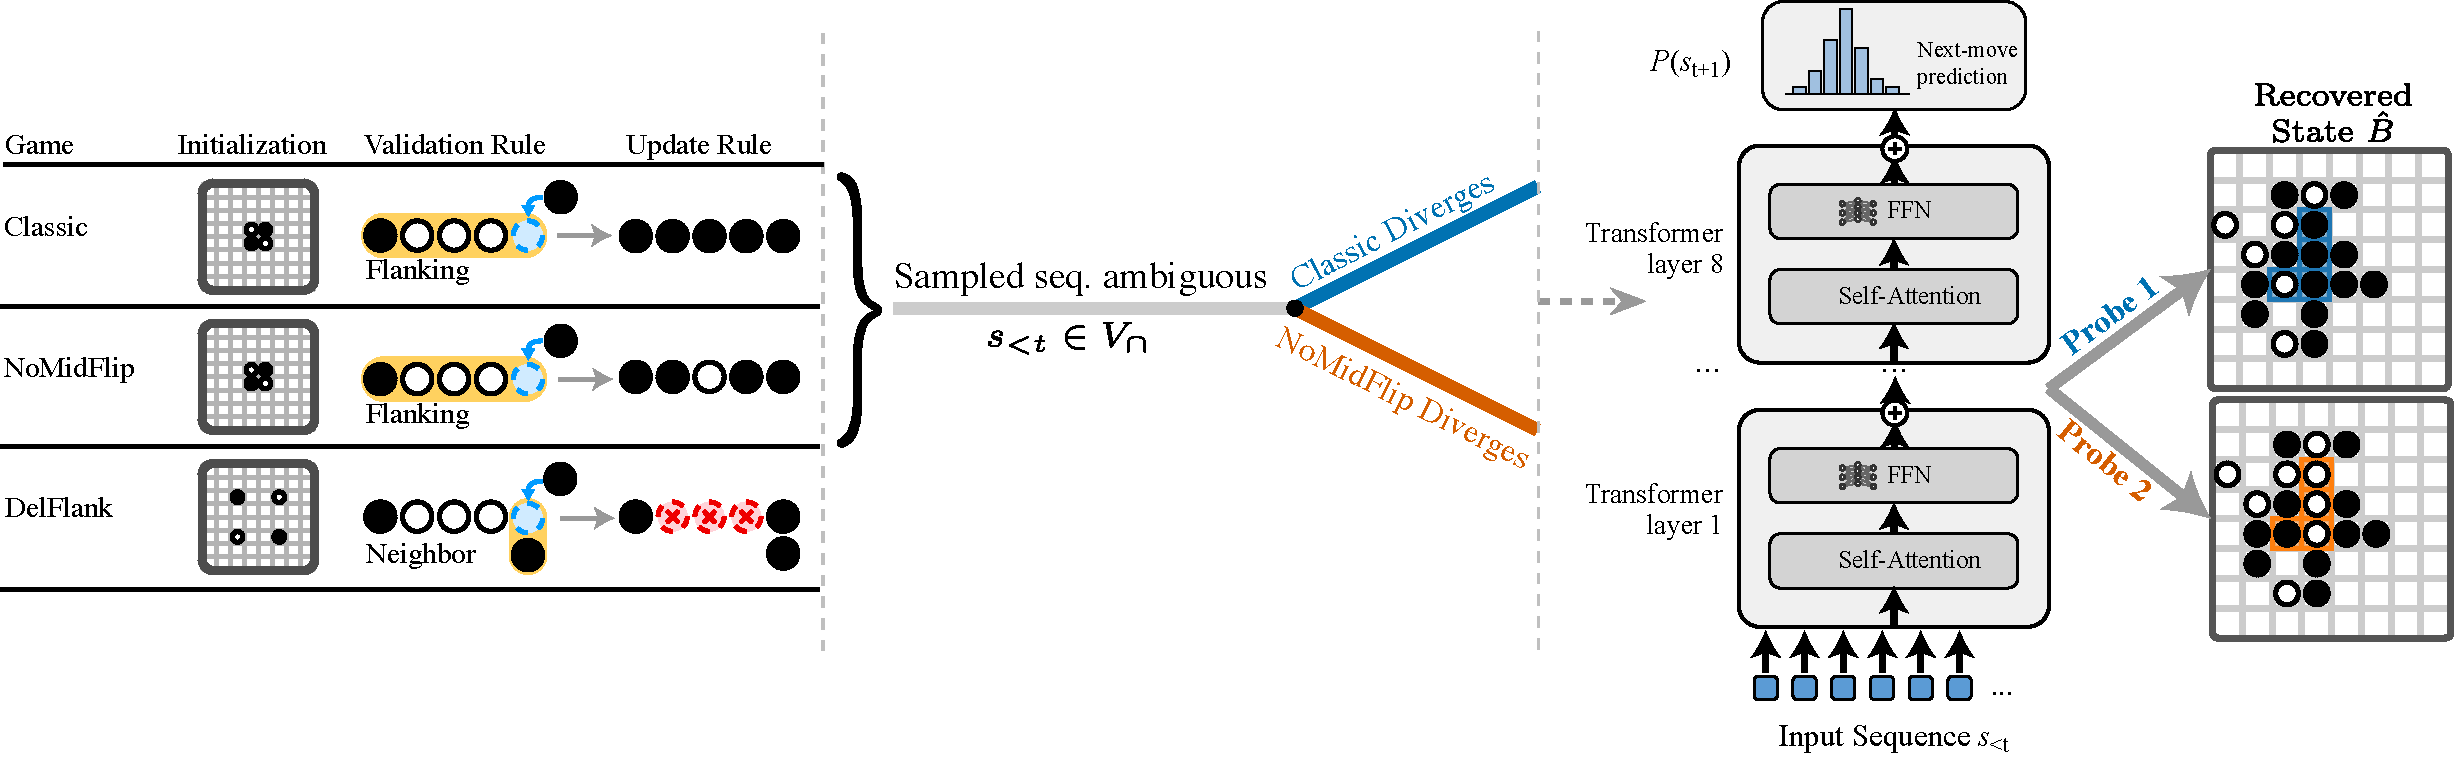
\includegraphics[width=\linewidth]{figures/fig1final.pdf}
        \caption{\textbf{The MetaOthello Framework.} (Left) We define a universe of games sharing a board size and vocabulary but differing in dynamics. (Middle) We sample sequences from these games. Early in the game, sequences are often valid under both rule sets (the ``Ambiguous'' branch), creating an informational conflict for the model. (Right) We train a small GPT model on these sequences and use Linear Probes on the residual stream to reconstruct the internal board representation.}
    \label{fig:metaothello_pipeline}
\end{figure*}

Large transformer models trained on diverse data must handle multiple generative processes. One model must translate languages, debug code, solve arithmetic, and it must determine which sort of text to simulate based on context \cite{merullo_circuit_2024, todd_function_2024}. Mechanistic interpretability has made strides in understanding how models represent individual concepts \cite{park_geometry_2024}, and implement specific tasks \cite{wang_interpretability_2022}, including evidence of emergent internal state-tracking (``world models'')\footnote{Following \citet{li_what_2025}, we use 'world model' to mean a causally complete representation—one sufficient to reconstruct the latent state of the data-generating process, without implying the model 'understands' that state.}  Yet these analyses study one task at a time. Real models face heterogeneous data where multiple rule systems coexist—and may conflict. This raises a question: how does a single transformer organize multiple world models within a shared representation space in Othello-GPT and related systems \cite{li_emergent_2024, nanda_emergent_2023}.

Addressing this question in large-scale models is challenging due to the difficulty of isolating specific rule systems in naturalistic data. We address this gap with \textit{MetaOthello}, a toy-model framework for generating variants of Othello that share a common syntax (an $8 \times 8$ board) but differ in their underlying physics (update rules and validity logic). We train small transformers on ``pure'' datasets generated by a single game, and ``mixed'' datasets generated by sampling from a pair of variants.

Our main findings are: 

\textbf{Cross-variant alignment.} Transformers trained on heterogeneous game data do not partition their capacity into isolated sub-models. Instead, board-state representations learned for one game transfer causally to others. Linear probes trained on one variant can intervene on another's internal state with effectiveness approaching matched probes. 

\textbf{Syntax invariance.} For isomorphic games with scrambled tokenization, representations are equivalent up to a single orthogonal rotation that generalizes across layers---demonstrating the model learns abstract structure independent of surface tokens. 

\textbf{Layerwise routing and economization.} When rules partially overlap, early layers track game-agnostic board state while a middle layer identifies game identity; later layers apply game-specific rules. The model economizes by keeping representations shared where games overlap, diverging only where rules explicitly conflict.

These results suggest that transformers converge on aligned state representations across world models while maintaining independent game-specific computations. We view MetaOthello as a methodological contribution: a controlled testbed for developing and validating interpretability techniques that may eventually scale to understanding how larger models organize heterogeneous knowledge.

\section{Related Work}


\paragraph{Emergent world models in sequence models.} Whether sequence models truly learn causal world representations or just surface statistics remains debated. \citet{li_emergent_2024} demonstrated that probes can decode true board states from activations of models trained on Othello sequences, and that interventions on these activations causally shift the model predictions. Building on this, \citet{nanda_emergent_2023} showed linear probes suffice when classifying tiles as ``mine/yours/empty'' rather than absolute colors, enabling intervention via simple vector addition. Subsequent work provides strong replication across architectures \cite{yuan_revisiting_2025}, circuit-level analysis with sparse autoencoders \cite{wong_othellogpt_2025}, and causal interpretations of attention \cite{rohekar_causal_2025}. Beyond Othello, similar world models appear in chess \cite{karvonen_emergent_2024} and in LLMs' representations of space and time \cite{gurnee_language_2023}. \citet{richens_general_2025} prove theoretically that goal-directed agents must contain world models.

\paragraph{Multi-task representation learning.} How one set of weights encodes many tasks is an emerging question. The superposition hypothesis suggests models compress features into polysemantic neurons \cite{elhage_toy_2022}. Task vectors show distinct skills correspond to separable directions in weight space that compose arithmetically \cite{ilharco_editing_2023}; function vectors extend this to activation space during in-context learning \cite{todd_function_2024}. \citet{vafidis_disentangling_2025} show multi-task agents develop representations where latent factors align along orthogonal directions. The Platonic Representation Hypothesis conjectures that diverse training drives convergence toward geometrically isomorphic representations across tasks \cite{huh_platonic_2024}.

Most relevant to our work, \citet{hua_mothello_2024} train on multilingual Othello sequences (mOthello), finding cross-vocabulary alignment requires shared ``anchor tokens.'' However, mOthello varies vocabulary while holding rules fixed—testing cross-lingual transfer, not multi-rule arbitration. MetaOthello fills this gap by varying the rules themselves: the same move sequence produces different board states under different update rules, creating genuine conflicts in latent state that neither world-model nor multi-task research has previously examined.

\section{MetaOthello}
MetaOthello is a framework defining a class of games played on an $8 \times 8$ board in which each of the 64 tiles can have one of three states at any time- $\texttt{white}$, $\texttt{black}$, or $\texttt{empty}$. We label a unique state of the board $B \in \mathcal{B} = \{\texttt{white}, \texttt{black}, \texttt{empty}\}^{64}$. The set of possible moves for the current player, including `pass' or $\varnothing$, is $M = \{\varnothing, (1,1), \ldots, (8,8)\}$. Since the board has 64 tiles, the size of the move set $|M| = 64$ (or $65$, including $\varnothing$ if no move is possible). A game, g, which is an instance of MetaOthello, is defined as the triplet $g = (B_0, V, U)$
where $B_0$ is a starting board state, $V$ is a validation rule, and $U$ is an update rule. A validation rule maps board states to sets of legal next moves: $V : \mathcal{B} \mapsto P(M)$, where $P(M)$ is the power set of $M$. An update rule maps a move applied to a board state to the resultant board state (for instance, after flanked chips are flipped): $U : M \times \mathcal{B} \mapsto B.$

We call the set of all possible sequences generated by a game $S(g)$. Given a game $g$ and a sequence of moves $s \in S(g)$, we can refer to the board state $B_k$ after these moves as $B(s, g)$. If $s \notin S(g)$ then $B(s, g) = \varnothing$. We use a shorthand to refer to the set of legal moves at turn $k+1$ after sequence $s$ in $g$ as $V(s, g)  = v(B(s, g))$, where again $v(\varnothing) = \varnothing$.

\subsection{MetaOthello Variants}

We introduce two Othello variants to create mixed-game datasets: one highly similar (high game-tree overlap) and one dissimilar: 

\textit{NoMidFlip:} Same initialization and validation rules as Classic, but the update only flips the outermost two flanked tiles.

\textit{DelFlank:} Open spread initialization instead of central; this variant employs a \textit{neighbor validation rule}: a move is valid if and only if it is adjacent to at least one piece of the current player's color; and the update differs in that flanked pieces are deleted rather than flipped.

These variants are visualized in Figure \ref{fig:metaothello_pipeline}. Both games generate sequences of moves that are illegal in standard Othello. NoMidFlip behaves similarly to standard Othello: the number of playable moves rises and then falls as the board fills up. DelFlank allows for games much longer than 60 because tiles can be deleted, and its game tree is consequently much larger at every depth. In either case the termination condition can trigger prior to 60 moves.

\textit{Iago:} To distinguish between the model's ability to learn specific game rules versus its ability to form abstract structural representations, we introduce a scrambled variant of Othello. We define the Token Space $\mathcal{T} = \{0, 1, \ldots, 63\}$ as the vocabulary of the model, distinct from the Move Space $M$ (the geometric coordinates on the board). A game $g$ is now equipped with a Syntax Map $\phi_g: \mathcal{T} \to M$, a bijection that maps an arbitrary token $t$ to a physical move $m$. We define the Iago experimental setup as a pair of games $G_{\text{Iago}} = \{g_{std}, g_{scr}\}$ which share identical logic but possess orthogonal syntax maps. This allows us to test whether the model learns a shared latent world model $W$ such that $W(s_{\text{classic}}) \approx W(s_{\text{iago}})$ despite the disjoint input vocabularies.

\section{Model Training \& Evaluation}
\subsection{Synthetic Data}
We create \textit{pure} and \textit{mixed-game} datasets by sampling sequences either from a single game or from one of two games. In all tests, the games used are Classic, NoMidFlip, DelFlank, and Iago. All game sequences are capped at $T_{max} = 60$. We train single-game models on datasets of $20M$ sequences and mixed-game models on datasets of $40M$ sequences ($20M$ from each).

\subsection{Model Parameterization}
We follow previous work on Othello-GPT by using an 8-layer Transformer ($L=8$) with 8 attention heads per layer ($H=8$) and an embedding dimension of $d_{\text{model}} = 512$ \cite{li_emergent_2024}. The context window size ($T$) was set to 59 tokens, corresponding to the maximum length of a transcript in our dataset (60).

We train the specified decoder-only Transformer model for 250 epochs each. Table \ref{tab:alpha_scores} shows each trained model's performance. To enable fair comparison of performance across different games, we created a tailored performance metric described in the following section.


\subsection{Evaluation}
We propose a metric for model performance $\alpha(\theta \mid s)$ that (a) accounts for the best possible performance given an input sequence $s$, which would be a loss just equal to the entropy $H_G(s)$, i.e. zero excess entropy; and (b) also accounts for the loss due to random guessing, i.e. the excess entropy if the model were purely random. The second requirement arises because some games have larger next-move sets on average, and a random predictor will be inaccurately rated as higher-performing in those games unless we adjust for the size of the valid move set.
\begin{equation}
    \alpha(\theta \mid s) = 1 - \dfrac{D_\text{KL}(P\mid \mid Q_{\theta})}{D_\text{KL}(P \mid \mid U)}
\end{equation}
where $U$ denotes a uniform distribution over the entire move set $M$. This normalized KL divergence is equal to $1$ when the loss is minimized and $0$ when it is equivalent to a uniform distribution, i.e., random guessing. The $\alpha$ score bears the additional benefit that it can compare outputs $Q_\theta$ to an arbitrary complex ground truth distribution $P$, e.g., in the case where $s$ comes from one of 2 or more games, which may have different prior probabilities $P(g_i)$.

\section{Results}

\subsection{Model Performance \& Probe Validation}
We first confirm that pure- and mixed-game models exhibit the same baseline interpretability properties as standard Othello-GPT. All models achieve near-optimal prediction, with $\alpha > 0.98$ across the board. Performance dips by about half a percentage point in mixed models as compared to their single-game alternates, particularly in the second half of the game (see Appendix Figure \ref{fig:alpha_scores}). Second, generalizing the result from \citealt{nanda_emergent_2023}, we show that linear probes can accurately infer values of ``mine,'' ``yours,'' and ``empty'' at each board position for each game type (Appendix Figure \ref{fig:probe_acc}). Probes trained on earlier layers and on mixed models show worse performance than those trained on later layers and single-game models.

\begin{table}
\centering
\small
\caption{Model Performance: We measure model performance using the $\alpha$ metric to ensure comparability across games. All models perform well, with $\alpha=1$ indicating perfect overlap between the model's predicted probabilities and the ground truth.}
\label{tab:alpha_scores}
\begin{tabular}{p{3cm} p{1.5cm} c}
\hline
\textbf{Model Name} & \textbf{Game} & \textbf{Avg. $\alpha$ Score $\pm$ CI} \\ \hline
Classic & Classic & $0.995 \pm 0.002$ \\
Nomidflip & Nomidflip & $0.988 \pm 0.003$ \\
Delflank & Delflank & $0.997 \pm 0.001$ \\
Iago & Iago & $0.994 \pm 0.002$ \\
Classic-Nomidflip & Classic & $0.991 \pm 0.003$ \\
Classic-Nomidflip & Nomidflip & $0.983 \pm 0.004$ \\
Classic-Delflank & Classic & $0.992 \pm 0.002$ \\
Classic-Delflank & Delflank & $0.995 \pm 0.002$ \\
Classic-Iago & Classic & $0.992 \pm 0.003$ \\
Classic-Iago & Iago & $0.991 \pm 0.003$ \\
Nomid-Delflank & Nomidflip & $0.984 \pm 0.004$ \\
Nomid-Delflank & Delflank & $0.996 \pm 0.002$ \\ \hline
\end{tabular}
\end{table}

\begin{figure*}[htbp]
    \centering
    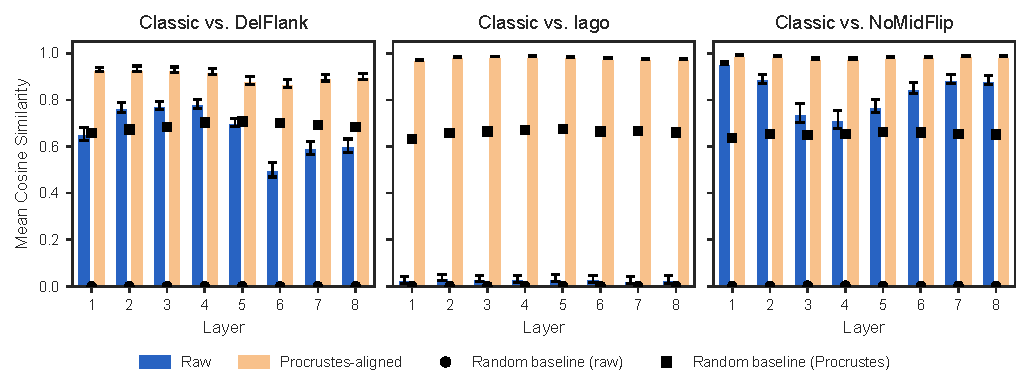
\includegraphics[width=\linewidth]{figures/probe_weight_similarity/cosine_sim_aggregated.pdf}
        \caption{Cosine similarity between board state probe weights in mixed models, with random baseline controls. Blue bars show raw cosine similarity; orange bars show similarity after per-layer Procrustes alignment. Black circles and squares indicate expected similarity for random probes (shuffled to preserve distribution) before and after alignment, respectively. For Classic vs. Iago (center), raw similarity matches the random raw baseline (0.03). However, after alignment, similarity reaches 0.98—substantially exceeding the random Procrustes baseline of 0.68. Error bars denote 95\% CIs across 192 probe dimensions.}
        \label{fig:probe_sim_rand}
\end{figure*}

\subsection{Cross-variant alignment of board-state features}
Given that mixed-game models linearly encode board states for all variants, we investigate their internal organization: does the model partition its residual stream into distinct subspaces for each game, or does it utilize a shared representational format? We first examine this question for rule-modified variants (NoMidFlip, DelFlank), then separately for the tokenization-scrambled variant (Iago), which requires distinct methodology.

\subsubsection{``Platonic'' Board Representation Geometry}

We first evaluate the similarity of the linear probes trained for each game variant. Each board state probe consists of a $\mathbb{R}^{192 \times 512}$ matrix in which each row corresponds to a vector $w_{i,c}$ which represents a direction in the activation space corresponding to a specific board feature (e.g., ``tile C3 is Mine''). We pair probe weights from Classic and variant probes trained on the mixed-model residual stream and calculate their cosine similarities, yielding 192 values per layer. Figure \ref{fig:probe_sim_rand} reports averages and 95\% confidence interval; individual tile-level values appear in Appendix Figure \ref{fig:tile_cosine}.

\paragraph{Probe weight alignment methodology.}
To assess whether probe weights encode the same features up to a rotation, we compute per-layer Procrustes alignment:
for each layer $\ell$, we find the orthogonal matrix $\mathbf{R}^{\ell} \in \mathbb{R}^{512\times512}$ that best aligns
$W^{\ell}_{\text{Classic}}$ to $W^{\ell}_{\text{Variant}}$ via SVD of
$\bigl(W^{\ell}_{\text{Variant}}\bigr)^\top W^{\ell}_{\text{Classic}}$.
We then report cosine similarities between corresponding rows of
$W^{\ell}_{\text{Classic}}$ and $W^{\ell}_{\text{Variant}}$.
Since we compare learned parameters rather than model outputs, no train/test split is required.

For Classic vs. NoMidFlip, we observe high raw cosine similarity ($\approx 0.95$) in early and later layers where Procrustes alignment yields only modest further improvement ($\lesssim 0.05$). For Classic vs. DelFlank, raw similarity is moderate ($\approx 0.67$), but Procrustes alignment moves it to $> 0.90$ across the majority of layers. Both aligned similarities substantially exceed the random baseline ($\approx0.68$ for Procrustes-aligned random matrices; Figure 2), confirming that the geometric correspondence reflects learned structure rather than high-dimensional coincidence.

\subsubsection{Causal Efficacy and Cross-Probe Intervention}
Representational similarity alone does not prove that the model uses these features in the same way. To test the functional equivalence of these board state representations, we perform a cross-probe intervention experiment.

We replicate the causal intervention from previous work on Othello-GPT \cite{nanda_emergent_2023, li_emergent_2024}. We use the probe weights to intervene on the board state, $B$, to convince the model that the board state is altered, $B'$. We alter the board state by either flipping the piece from ``mine'' to ``yours'' or vice-versa or by erasing it from the board. Concretely, we accomplish this by adding the corresponding probe weight vector to the activations $h_l(s)$ at each layer: 
\begin{equation}
    h_l(s) \rightarrow h_l(s) + \gamma w^{l}_{i,c}
\end{equation}
where $\gamma$ is a scaling factor and $i, c$ index the tile and its post-intervention state. Following \cite{nanda_emergent_2023} we apply this steering across all eight layers at once. \footnote{All-layer intervention maximizes steering strength but may over-intervene. $\gamma = 5$ for current work, but is not fully optimized. Single-layer ablations and potential compensation effects \citep{mcgrath_hydra_2023} remain open for circuit-level analysis; Section 5.4 partially addresses layer specificity.} We then compute the error rate, the number of false positives and false negatives for top-$k$ predictions. 

As shown in Figure \ref{fig:probe_intervention_global}, cross-probe interventions (hatched coral bars) are nearly as effective as ``correct-probe'' interventions (blue bars) at steering the model's predicted board state. This dissociation between raw representational similarity and causal efficacy is notable: even when probe similarity is moderate (as in Classic–DelFlank), the Classic probe can intervene on DelFlank boards with comparable accuracy.

\begin{figure}[htbp]
    \centering
    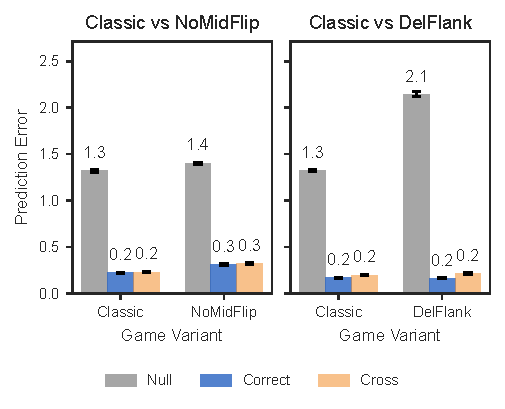
\includegraphics[width=\linewidth]{figures/intervention_evaluation/intervention_global_comparison.pdf}
    \caption{Global intervention error across conditions. Gray bars show null baseline (no intervention); blue bars show correct-probe intervention; orange bars show cross-probe intervention. Error bars denote 95\% CI. We see that cross-probe intervention is nearly as effective as the correct probe in steering board states.}
    \label{fig:probe_intervention_global}
\end{figure}
\subsection{Syntax Invariance: The Iago Experiment}

The preceding analyses examined games sharing tokenization but differing in rules. We now ask the complementary question: when games are computationally isomorphic but use permuted token vocabularies, does the model still learn a shared latent representation?

\paragraph{Probe weight analysis.} Raw cosine similarity between Classic and Iago probes is indistinguishable from a random baseline ($\approx 0.03$; Figure~\ref{fig:probe_sim_rand}, center). However, after per-layer Procrustes alignment, similarity reaches 0.98---substantially exceeding the random-alignment baseline of 0.68. The model learns the same latent structure for both games, differing only by a rotation induced by the input vocabularies.

\paragraph{Residual stream alignment.} We test whether this rotational equivalence extends to the full residual stream. We estimate a single global transformation $\Omega \in \mathbb{R}^{512 \times 512}$ via orthogonal Procrustes on paired Classic/Iago activations, pooling across all layers and positions, on a training set. 

We then feed a test set of Classic sequences into the mixed model, apply $\Omega$ at a specific intervention layer $\ell'$, and measure performance on corresponding Iago moves. As shown in Figure~\ref{fig:classic_iago_intervention}, intervening at any layer (except for 8) recovers near-baseline Iago performance. This is much higher than accuracy of Iago moves on Classic sequences ($\alpha \approx -2.9$)

\begin{figure}[htbp]
    \centering
    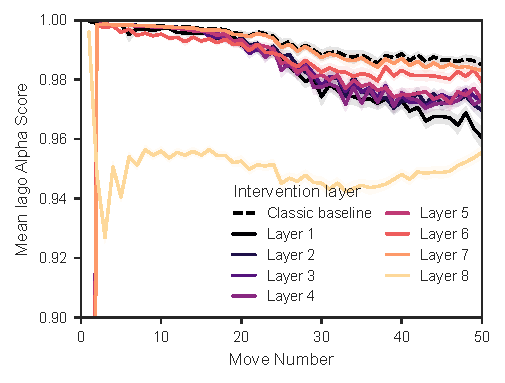
\includegraphics[width=\linewidth]{figures/iago/iago_alignment.pdf}
    \caption{Classic-to-Iago activation alignment via orthogonal Procrustes. We feed Classic sequences to the mixed Classic-Iago model, apply a learned orthogonal rotation $\Omega$ to the residual stream at layer $l'$, and measure how well the model predicts corresponding Iago moves ($\alpha$ score).}
    \label{fig:classic_iago_intervention}
\end{figure}

These results suggest that the transformer’s board-state representations are largely syntax-invariant up to a token permutation. The same abstract state geometry can be recovered via an approximately orthogonal transformation. Importantly, this observation alone does not determine how such invariance is implemented internally. The aligned geometry could reflect a single shared representation or multiple representations with similar structure, or something more nuanced. Our results therefore support representational isomorphism across syntaxes, but stop short of establishing whether the model maintains one shared world model or multiple distinct instantiations with similar structure.


\begin{figure*}
    \centering
    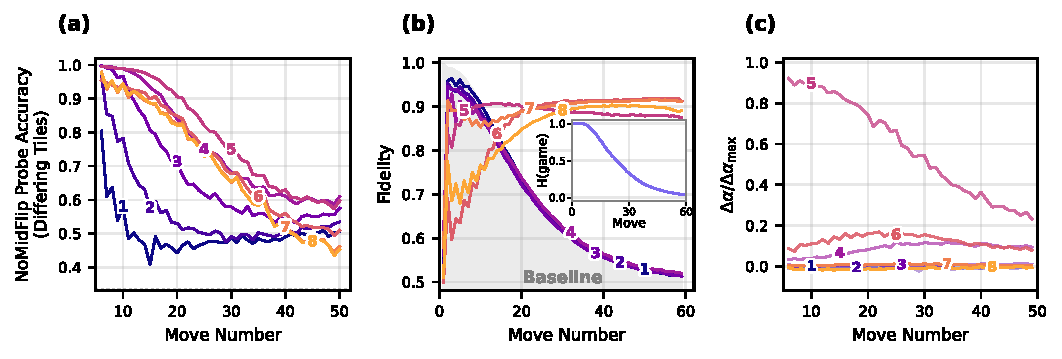
\includegraphics[width=\linewidth]{figures/figure5_combined.pdf}
    \caption{\textbf{Differentiation dynamics in the Classic--NoMidFlip mixed model.} (a) performance of NoMidFlip probes on tiles that differ between NoMidFlip and Classic after an ambiguous sequence $s^*$. (b) Probe Fidelity: Probes trained to estimate the probability of the game context ($P(\text{Classic})$) where fidelity is ($1 - |P_{\text{probe}} - P_{\text{GT}}|$). We also train a ``Baseline'' probe on one-hot encoded $60 \times 60$ (move $\times$ move number) inputs. Inset: Average entropy of the ground truth game distribution $P(g|s_{<t})$ over time. (c) Causal Steering: Injecting a game-steering vector ($\lambda[\mu_{\text{NoMid}} - \mu_{\text{Classic}}]$) to measure the change in adherence to NoMidFlip rules, measured by the normalized increase in $\alpha$-score relative to NoMidFlip-valid moves.}
    \label{fig:divergence_dynamics}
\end{figure*}

\subsection{How do the models handle ambiguous sequences?}

Results from the previous section indicated that although the Classic and DelFlank/NoMidFlip board representations differ substantially for particular tile locations, states, and layers, intervening on the variant representation can still causally influence the Classic next token predictions approximately as well as intervening on the Classic representation. As we indicate in the prior section, it is tempting to interpret this as causal evidence for the existence of a single shared linear board state representation in the model: a so-called ``Platonic'' representation \cite{huh_platonic_2024}. But in the mixed game context -- particularly Classic-NoMidFlip -- this result raises a conundrum. There are many sequences $s^*$ present in the languages of both games which generate nonequal board states and different valid move sets:
\[
B(s^*, g_1) \neq B(s^*, g_2), \qquad V(s^*, g_1) \neq V(s^*, g_2).
\]
We call these \textit{ambiguous} sequences. For the model to perform well on these sequences, it must predict a weighted combination of next tokens drawing on the board states of \textit{both} games, even though the prior results seem to show that there is effectively a single \textit{causal} board state representation. Note that optimal prediction of a next token $x$ for ambiguous sequences under the cross entropy loss is:
\begin{align}
    P(x \mid s^*, \{g_1, g_2\})
        &= P(g_1 \mid s^*) \frac{\mathds{1}[x \in V(s^*, g_1)]}{|V(s^*, g_1)|} \nonumber \\
        &+ P(g_2 \mid s^*) \frac{\mathds{1}[x \in V(s^*, g_2)]}{|V(s^*, g_2)|}. 
\end{align}

In such cases of differing next move sets under $s^*$, how well does the model handle next-token prediction, how does it represent the board state(s), and how does it manage potentially conflicting representations? We start by investigating these questions in the Classic-NoMidFlip model, where ambiguity is common. We then move to the Classic-DelFlank model, which presents an interesting edge case because of the large difference in the sizes of the two games' languages.

\subsection{Diverging games: Steering vectors govern layerwise specialization}\label{ambiguity}

In the Classic--NoMidFlip model games share validation rules and board dimensions but differ in update dynamics. This setup creates wide-spread ambiguity: sequences often remain valid in both games until a specific move triggers the divergent update rules. This ambiguity can be quantified as the average entropy of the game identity conditionalized on a sequence sampled from the mixed game dataset,  $\mathbb{E}[H(g \mid s_{<t})]$; i.e. how uncertain we are on average about which game a sequence comes from, after seeing $t$ moves (Figure \ref{fig:divergence_dynamics}b, inset).

While Section 5.2 showed that Classic and NoMidFlip representations are causally interchangeable, they are not identical. We quantify this divergence by calculating, for each tile, the actual probability that its value will differ in Classic versus NoMidFlip for a randomly sampled ambiguous sequence $s^*$. We find that the representational dissimilarity correlates strongly with the probability of a tile difference, and this correlation gets stronger for higher layers, reaching $R^2 = 0.95$ at layer 8 (Appendix Figure \ref{fig:principal_angle_classic_nomid}). (Notably, this correlation spikes after layer 5, from $R^2_{L5} = 0.35$ to $R^2_{L6} = 0.73$.) In other words, the probability of a conflict between Classic and NoMidFlip on a given tile almost entirely predicts the cosine similarity between the corresponding representations of that tile's value by the last layer. We get qualitatively similar results by comparing the principal angles between the subspaces spanned by each position's $(v_{mine}, v_{yours})$ vectors for Classic vs. NoMidFlip: the more likely the games disagree at a board position, the higher the principal angle. This result holds strongly across all layers with $R^2 \in (0.70, 0.89)$ (Appendix Figure \ref{fig:principal_angle_classic_nomid}). Unsurprisingly, the ``Empty'' representations learned for each game are nearly identical in all probes, as playing a tile in either game permanently sets that location to a non-empty value. Overall, these findings present evidence that the model economizes on constructing dual world models, focusing the extra representational capacity where it is needed; i.e., where the two worlds are likely to diverge.

We also test all eight NoMidFlip board probes' ability to correctly recover tile values when they differ from the Classic rules value. We find that this accuracy declines approximately monotonically with move number, and that the layer 5 probe is consistently the most accurate across all move numbers (Figure \ref{fig:divergence_dynamics}a).

These results indicate that, for ambiguous sequences, the two board representations diverge so as to capture meaningful differences between the two corresponding board states.

Having found suggestive evidence that the model encodes board tile states differently in proportion to their probability of diverging, and continuing our work grounded in linearly decodable representations for causal analysis, we ask whether the model encodes a linear representation of the likelihood of each game $g_i$ given sequence $\Tilde{s}$. We train a linear probe to predict the Bayesian ground truth likelihood $P(g \mid \Tilde{s})$ from the activations $h_l(\Tilde{s})$ from each layer; we compare these probes to one trained on $60 \times 60$ vectors of one-hot encoded move-and-move-numbers, which serves as an analytic baseline. The latter probe's performance establishes how much information about the game identity is linearly encoded in the move sequence, prior to any processing by the model. We find that layers 1-4 perform no better than the baseline, while layers 5-8 contain a reliably 90\% accurate linear representation of the game likelihood (Figure \ref{fig:divergence_dynamics}b). In further tests (Figure \ref{fig:NMF-prob-collapse}), we find that when a move takes a sequence out of the Classic $\cap$ NoMidFlip game tree and into the Classic $\setminus$ NoMidFlip game tree, the probe's inferred probability of NoMidFlip drops to zero most reliably in layers 5 and 6, although this responsiveness decays with the length of the sequence.

We tested the causal role of these game probabilities using an intervention. We computed a difference vector $\Delta \mu = \mu_{\text{NoMid}} - \mu_{\text{Classic}}$ from the game ID probe weights and added it to the residual stream of sequences possible under both games (Figure \ref{fig:divergence_dynamics}c). Injecting $\Delta \mu$ into early layers (1--4) produces little-to-no change in model output, and injection at later layers (6--8) shows a similarly small effect. However, intervention at Layer 5 significantly increases the likelihood of NoMidFlip-consistent moves. Notably, this intervention is only associated with a negligible change in the fidelity of the downstream NoMidFlip board state representations, even when focused on the tiles that are different between the two games.

Together, these findings indicate that Layer 5 acts as a pivotal point where shared representations diverge into game-specific computations. However, they also reinforce a tension with prior results: the Classic and NoMidFlip board representations appear causally equivalent (Figure \ref{fig:probe_intervention_global}), but they also capture different information for ambiguous sequences $s^*$.

\subsection{Out-of-distribution world modeling}

DelFlank provides a useful foil to NoMidFlip because the DelFlank game tree is much larger: it scales exponentially with move number, while the NoMidFlip and Classic game trees scale subexponentially except in the mid game. This difference comes from DelFlank's more permissive validation rule and ability to delete tiles, reopening squares to move. As a result, while DelFlank and Classic share an intersection until at least move 50, it is a vanishingly small part of DelFlank's game tree, and the likelihood of DelFlank, given an observed sequence $s_{<t} \in$ Classic $\cap$ DelFlank, approaches zero very rapidly. This means that ambiguous sequences past length scale $t^* \approx 12$ are functionally absent from the training data: in this limited sense, they are ``out of distribution.'' (More precisely, of 20M random DelFlank training sequences, we expect $\sim 19,500$ to remain ambiguous at move 5, $\sim 19$ at move 10, and $\lesssim 1$ beyond move 12.) Furthermore, optimal performance for such sequences under the cross-entropy loss (i.e., maximizing $\alpha$) requires predicting as if the sequence comes from Classic, even though it is technically compatible with the DelFlank rule set.

In this context, we ask whether the Classic-DelFlank model nonetheless maintains a distinct representation of the DelFlank board corresponding to a sequence sampled from this intersection. It is important to note that, particularly for longer sequences, this representation would only be useful in extremely rare cases. We test this by assessing the accuracy of the DelFlank probes (which have high fidelity on random DelFlank games) on these sequences. We find that DelFlank board probe accuracy at Layer~5 drops to $\approx67\%$, compared to $\approx99\%$ for Classic probes on the same sequences. This suggests that the model's internal representation has effectively ``selected'' the Classic world model for these ambiguous inputs.

Next, we ask whether we can intervene on the model to shift its behavior toward the DelFlank interpretation. We apply a steering vector $\Delta\mu = \mu_{\text{DelFlank}} - \mu_{\text{Classic}}$ derived from game identity probes, analogous to the NoMidFlip intervention described above. Figure~\ref{fig:steering_delflank} shows the results. Intervening at early layers (2--3) produces a strong shift toward DelFlank-valid moves, achieving normalized $\Delta\alpha \approx 0.75$ at early move numbers (Panel~A). This effect declines as games progress, falling to $\Delta\alpha \approx 0.3$ by move~30. Notably, intervention at Layer~5---the critical layer for NoMidFlip steering---has essentially no effect ($\Delta\alpha \approx 0$).

Crucially, early-layer steering also improves the \textit{downstream} DelFlank board representation (Panel~B). Without intervention, the DelFlank probe at Layer~5 achieves only $67.1\%$ accuracy on ambiguous sequences. After steering at Layer~1, this accuracy rises to $77.4\%$ ($+10.3\%$); Layer~2 steering yields a similar improvement to $75.8\%$ ($+8.7\%$). This causal effect on downstream representations distinguishes DelFlank from NoMidFlip, where Layer~5 steering changed model outputs but did not improve board probe accuracy at later layers.

\begin{figure}[h]
    \centering
    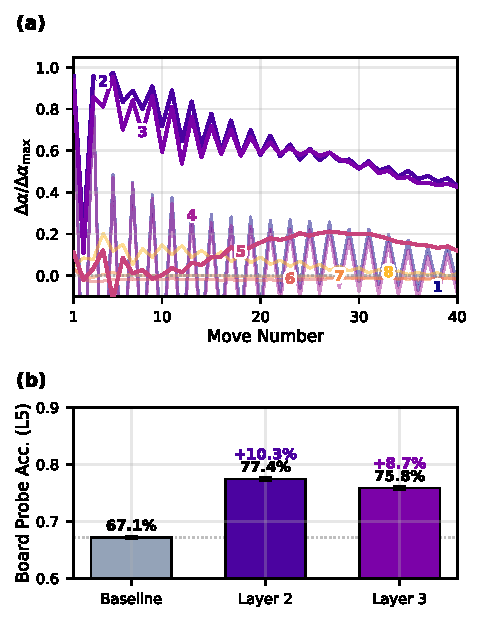
\includegraphics[width=0.85\linewidth]{figures/steering_delflank_combined.pdf}
    \caption{\textbf{Steering DelFlank on ambiguous sequences.} (A)~Normalized improvement in $\alpha$-score toward DelFlank-valid moves ($\Delta\alpha / \Delta\alpha_{\mathrm{max}}$) as a function of move number. Early layers (1--2) show strong steering effects that decline with game length; Layer~5 shows no effect. (B)~DelFlank board probe accuracy at Layer~5 under different steering conditions. Steering at early layers causally improves downstream representations, providing evidence for a selection mechanism distinct from NoMidFlip's subspace reweighting.}
    \label{fig:steering_delflank}
\end{figure}


\section{Conclusion} 

This study leverages the MetaOthello framework to demonstrate that transformers trained on heterogeneous generative processes do not partition their capacity into isolated sub-models. Instead, our findings suggest these models converge on a shared representation of state that is efficiently reused across contexts. Board-state representations are geometrically aligned across game variants: linear probes transfer causally between games with different update rules, and for syntax-scrambled variants (Iago), state representations are identical up to a single orthogonal rotation.

We also identify a distinct temporal structure in how the model manages conflicting rules: early layers track the shared board state, a middle layer identifies which game is being played, and later layers apply game-specific rules. The model economizes by keeping representations the same where games overlap, diverging only where rules explicitly conflict.

However, a key puzzle remains. While our tests show that board states from different games are causally interchangeable, the model still successfully distinguishes between games during ambiguous sequences where rules eventually diverge. The tension between a shared global representation and the need for local precision—suggests that linear analysis alone cannot fully explain the model's behavior, leaving an opening for future work on nonlinear mechanisms.

While this work uses a toy model, it offers significant methodological contributions to the field of mechanistic interpretability and the understanding of transformer models. By creating a controlled testbed where ground-truth latent states are known, MetaOthello allows researchers to validate interpretability techniques, such as probing and causal intervention.

Specifically, this research advances our understanding of how single models arbitrate between conflicting rule systems. The identification of specific ``routing'' layers that govern context switching suggests that complex multi-task behaviors may rely on identifiable, localized mechanisms rather than diffuse processing. These insights suggest how larger models may organize diverse knowledge and motivate more robust methods for analyzing internal state-tracking in general-purpose systems.

\section{Limitations}
Our findings are established in a controlled, synthetic setting and may not fully capture real-world multi-task learning. MetaOthello systematically varies rules and tokenizations, but remains far simpler than heterogeneous corpora where rule systems are implicit and numerous. We only test 50/50 mixtures, one 8-layer ($d_{\text{model}}=512$) architecture, and pairwise game mixtures, so the effects of imbalanced mixtures, scale, and many-way arbitration remain open. Finally, our analysis relies on linear probes; nonlinear structure and circuit-level analysis may reveal additional mechanisms.

\section*{Impact Statement}

This paper presents work whose goal is to advance the field of Machine Learning, specifically in the area of mechanistic interpretability. By establishing a controlled setting to study how models organize conflicting knowledge, this research contributes to the broader goal of making "black box" systems more transparent. Understanding how foundation models separate or merge different task contexts is a step toward verifying their safety and reliability in complex, real-world deployments. Beyond these contributions to model transparency and safety research, there are many potential societal consequences of our work, none of which we feel must be specifically highlighted here.


\bibliography{MetaOthelloGPT}
\bibliographystyle{icml2026}

\newpage
\appendix
\onecolumn
\section{Reproducibility}
\label{app:reproducibility}

\subsection{Data and Code Availability}
  \label{app:code}

  All code and pretrained assets are publicly available:
  \begin{itemize}
      \item \textbf{Code:} \url{https://github.com/aviralchawla/metaothello}
      \item \textbf{Models \& probes:} \url{https://huggingface.co/aviralchawla/metaothello}
      \item \textbf{Training data:} \url{https://huggingface.co/datasets/aviralchawla/metaothello}
  \end{itemize}
  The repository includes the MetaOthello game engine, data generation and model training scripts, board probe training and intervention analysis code, and all pretrained checkpoints. See
   the repository README for installation and reproduction instructions.

\subsection{Training Details}
\label{app:training}

\paragraph{Architecture.} All models use an 8-layer decoder-only Transformer with 8 attention heads per layer, embedding dimension $d_{\text{model}} = 512$ We use learned positional embeddings with a context window of $T = 59$ tokens. The vocabulary size is 66 (64 board positions plus a skip token and a pad token).

\paragraph{Optimizer.} We use AdamW \citep{loshchilov_decoupled_2019} with $\beta_1 = 0.9$, $\beta_2 = 0.99$, and weight decay $\lambda = 0.01$.

\paragraph{Learning rate.} We use a linear warmup over the first 1,000 steps to $5 \times 10^{-5}$ over the remaining training.

\paragraph{Batch size.} We use a batch size of 4096 sequences.

\paragraph{Training duration.} Single-game models are trained for 250 epochs on 20M sequences. Mixed-game models are trained for 250 epochs on 40M sequences. Training converges well before 250 epochs; we use this fixed budget for consistency.

\subsection{Probe Training Details}
\label{app:probes}

\paragraph{Architecture.} Linear probes are single-layer linear classifiers mapping from $\mathbb{R}^{512}$ to $\mathbb{R}^{3}$ (for mine/yours/empty classification) per board position, yielding 64 independent 3-way classifiers.

\paragraph{Training data.} Probes are trained on 100,000 sequences (sampled independently from model training data) with an 80/20 train/validation split.

\paragraph{Optimizer.} Adam with learning rate $3 \times 10^{-5}$, trained for 10 epochs with early stopping based on validation accuracy (patience = 5 epochs).

\paragraph{Game-identity probes.} These use the same architecture but predict $P(\text{game} \mid s_{<t})$ as a binary classification task, trained with cross-entropy loss against the Bayesian ground truth computed from Equation~\ref{eqn:posterior}.

\subsection{Random Seeds}
\label{app:seeds}

All model and probes training a fixed random seed (42) for reproducibility. Due to computational constraints the all models are only trained once.


\section{Model performance and $\alpha$ score}
\label{alpha-app}

Standard metrics such as cross-entropy loss or top-1 accuracy are insufficient for evaluating model performance in the MetaOthello setting. Because the size of the valid move set $|V(s, g)|$ varies significantly depending on the game variant $g$ and the game state $s$, the intrinsic entropy of the ground truth distribution fluctuates. A loss of 2.0 nats might represent perfect performance in a high-entropy state (many valid moves) but poor performance in a low-entropy state (forced move).

To address this, we introduce the $\alpha$-score, a normalized metric that measures how much of the reducible uncertainty the model has resolved, relative to a random baseline.

\subsection{Ground Truth Distribution in Mixed Environments}

In a mixed-game setting, the ground truth distribution over the next token $x_{t}$, given a history $s_{<t}$, is a mixture distribution marginalized over the set of possible games $\mathcal{G} = \{g_1, \dots, g_K\}$.

First, we define the likelihood of observing a sequence $s_{<t}$ under a specific game $g$. Assuming the data generation process samples move uniformly from the set of valid moves $V(s_{<k}, g)$ at each step $k$, the likelihood is the product of the inverse valid move set sizes:

\begin{equation}
    P(s_{<t} \mid g) = \prod_{k=0}^{t-1} \frac{1}{|V(s_{<k}, g)|} \cdot \mathbb{I}[s_k \in V(s_{<k}, g)]
\end{equation}

where $\mathbb{I}[\cdot]$ is the indicator function, which is $0$ if a move is illegal in game $g$.

We define the posterior probability that the current sequence is being generated by game $g$ using Bayes' theorem. Let $P(g)$ be the prior probability of sampling game $g$ (in our mixed datasets, $P(g) = 0.5$). The posterior is:

\begin{equation}
    P(g \mid s_{<t}) = \frac{P(s_{<t} \mid g) P(g)}{\sum_{g' \in \mathcal{G}} P(s_{<t} \mid g') P(g')}
    \label{eqn:posterior}
\end{equation}

Substituting the likelihood from Eq. \ref{eqn:posterior} we obtain the formulation described in the main text: the probability of a game is proportional to the product of the inverse valid move set sizes along the sequence.

Finally, the ground truth probability of the next token $x_t$ is the expectation over the game posteriors:

\begin{equation}
    P_{\text{GT}}(x_t \mid s_{<t}) = \sum_{g \in \mathcal{G}} P(x_t \mid s_{<t}, g) P(g \mid s_{<t})
\end{equation}

where $P(x_t \mid s_{<t}, g) = |V(s_{<t}, g)|^{-1}$ if $x_t$ is valid in $g$, and $0$ otherwise.

\subsection{The \texorpdfstring{$\alpha$}{alpha}-Score Definition}

We seek a metric $\alpha(\theta \mid s)$ that quantifies the model $Q_\theta$'s proximity to $P_{\text{GT}}$. We define two reference divergences:
\begin{enumerate}
    \item \textbf{Model Divergence:} $D_{\text{KL}}(P_{\text{GT}} \parallel Q_\theta)$, the excess entropy of the model relative to the ground truth.
    \item \textbf{Random Baseline Divergence:} $D_{\text{KL}}(P_{\text{GT}} \parallel U)$, the excess entropy of a uniform distribution $U$ (random guessing over the vocabulary) relative to the ground truth.
\end{enumerate}

The $\alpha$-score is defined as:

\begin{equation}
    \alpha(\theta \mid s) = 1 - \frac{D_{\text{KL}}(P_{\text{GT}} \parallel Q_{\theta})}{D_{\text{KL}}(P_{\text{GT}} \parallel U)}
\end{equation}

This metric has the following desirable properties:
\begin{itemize}
    \item $\alpha = 1$: The model perfectly matches the ground truth mixture distribution ($Q_\theta = P_{\text{GT}}$). This implies the model has perfectly disentangled the ambiguous games or perfectly modeled the superposition.
    \item $\alpha = 0$: The model performs equivalent to random guessing over the vocabulary.
    \item $\alpha < 0$: The model is being confidently wrong (assigning low probability to valid moves).
    \item It is naturally extensible to other comparisons besides the uniform distribution $U$; for instance, in a mixed game setting, we could replace $U$ with the distribution of next moves according to one of the two games.
    \item Crucially, $\alpha$ allows us to compare performance across games with vastly different branching factors (e.g., Delflank vs. NoMidFlip) on a unified scale.
\end{itemize}


\begin{figure}
    \centering
    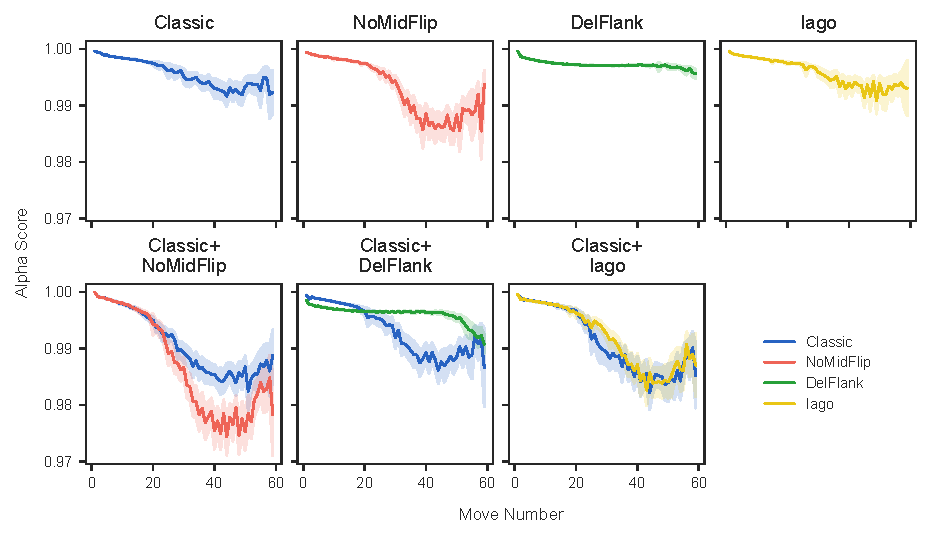
\includegraphics[width=0.9\linewidth]{figures/model_accuracy/model_accuracy_over_moves_alpha.pdf}
    \caption{Alpha scores of all models for sequences sampled from each game, shown as a function of move number with 95\% intervals.}
    \label{fig:alpha_scores}
\end{figure}

\section{Probe performance}

\begin{figure}[H]
    \centering
    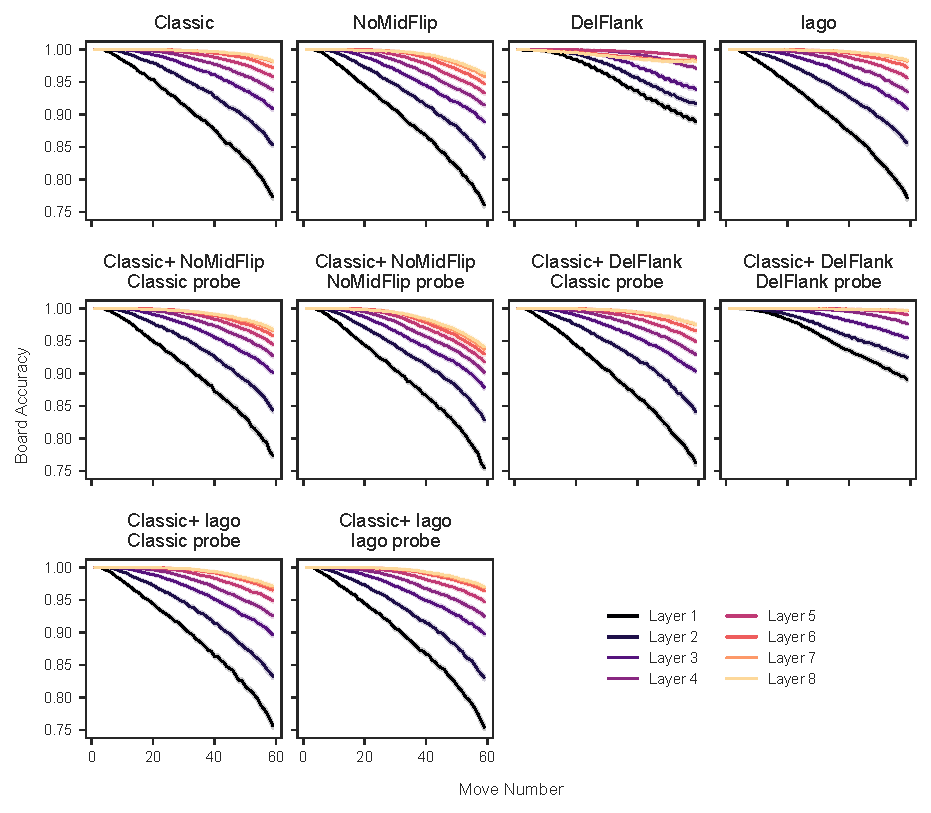
\includegraphics[width=0.9\linewidth]{figures/board_probe_accuracy/board_probe_accuracy_over_moves.pdf}
    \caption{Accuracies of linear probes trained to detect board states from model activations.}
    \label{fig:probe_acc}
\end{figure}


\begin{figure}
    \centering
    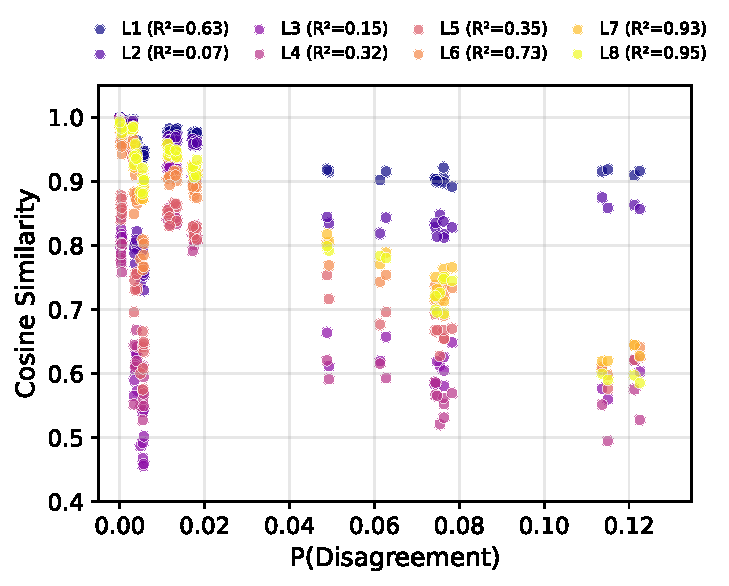
\includegraphics[width=0.49\linewidth]{figures/disagreement_vs_cosine_combined_Classic_NoMidFlip.pdf}
    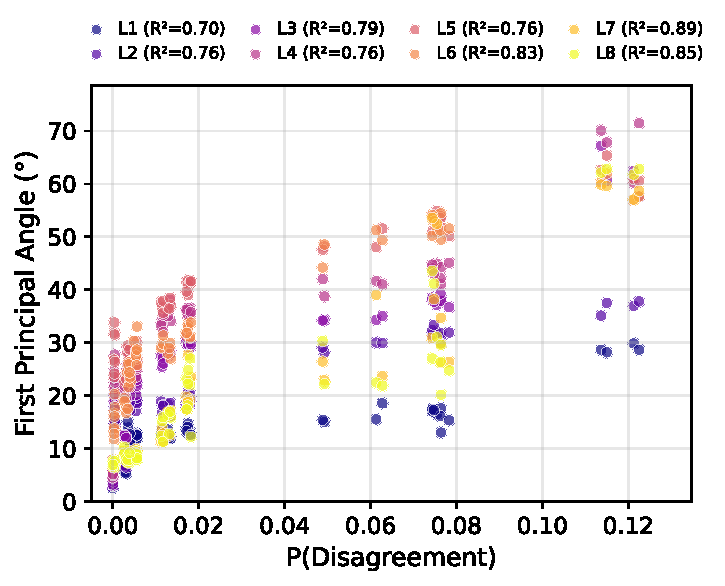
\includegraphics[width=0.49\linewidth]{figures/disagreement_vs_principal_angle_combined_Classic_NoMidFlip.pdf}
    \caption{(Left) Cosine similarity and (Right) Principal angle (deg.) between Classic and NoMidFlip tile-state representations, plotted against the actual probability that a given tile will have a conflicting state under the two rules.}
    \label{fig:principal_angle_classic_nomid}
\end{figure}

\begin{figure}
    \centering
    
    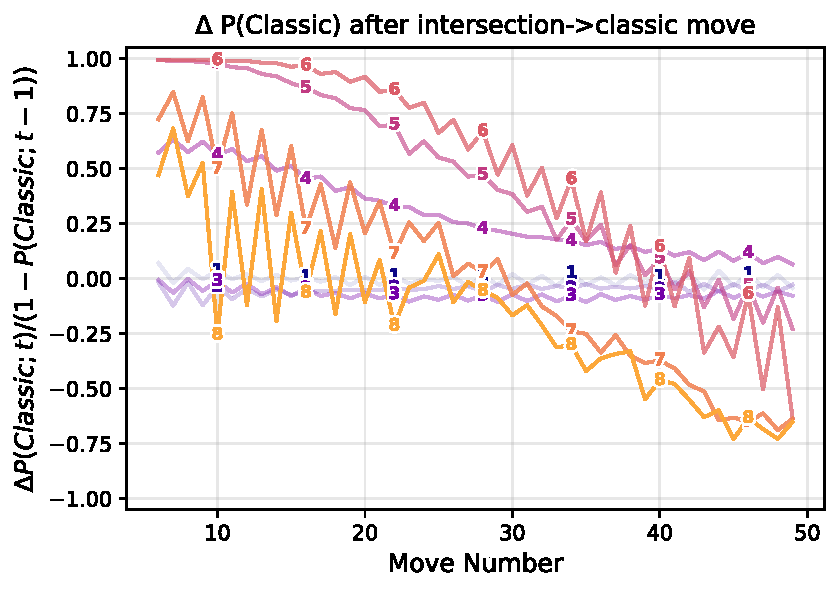
\includegraphics[width=0.5\linewidth]{figures/prob_collapse_NoMidFlip.pdf}
    \caption{Change in inferred $P(\text{Classic}|s)$ after playing a move only legal under Classic rules at the end of an ambiguous sequence $s^*$. Under optimal behavior, the probability of NoMidFlip should collapse to 0 and the probability of Classic to 1; we ask how close the inferred probability gets, compared to its value prior to this move.}
    \label{fig:NMF-prob-collapse}
\end{figure}


\begin{figure}
    \centering
    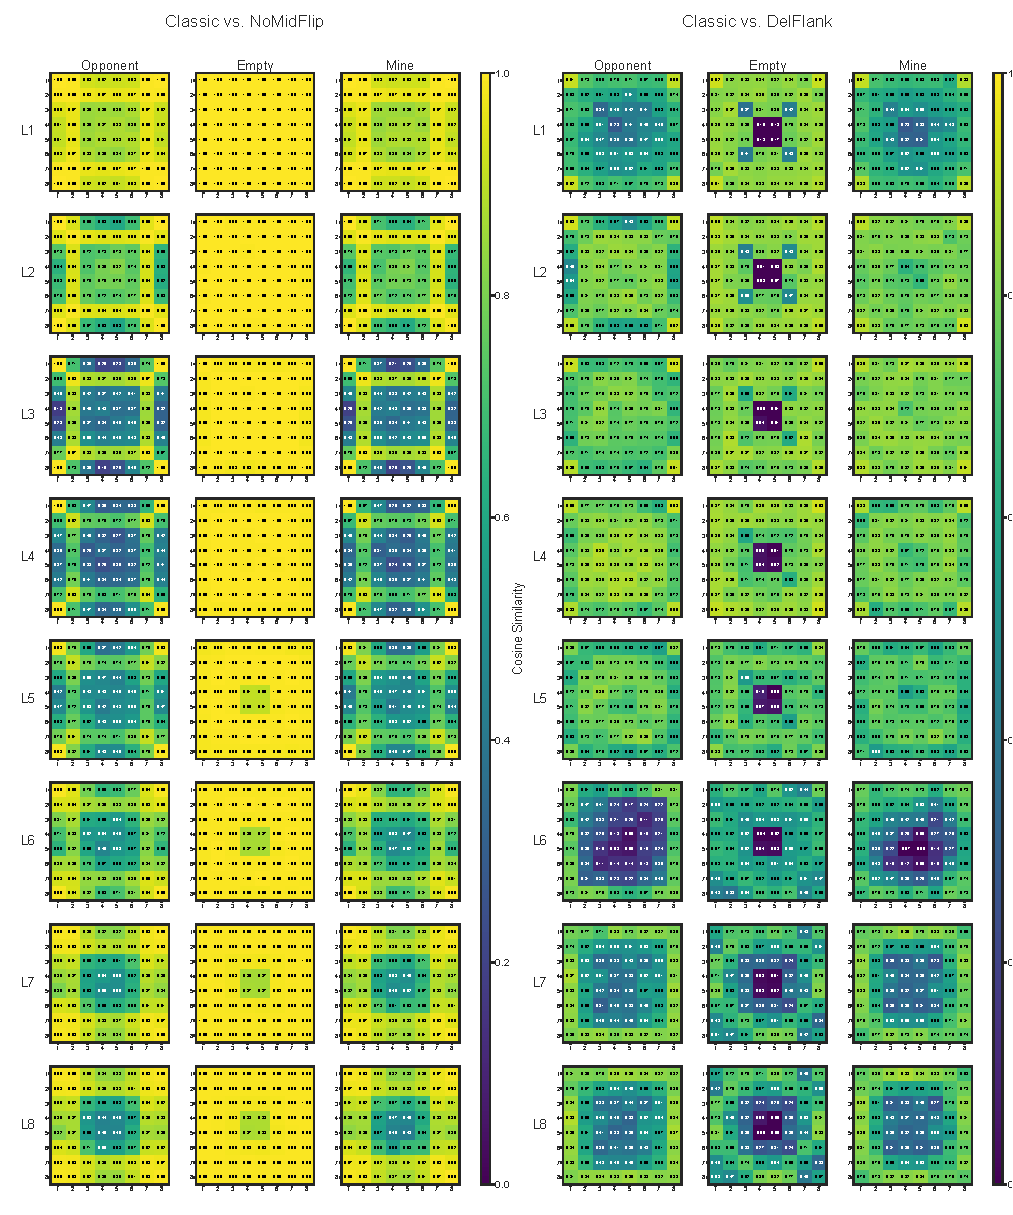
\includegraphics[width=\linewidth]{figures/probe_weight_similarity/tile_state_similarity.pdf}
    \caption{Cosine similarity of tile-state representations from each layer's probe for Classic and NoMidFlip (Left) and Classic and DelFlank (Right).}
    \label{fig:tile_cosine}
\end{figure}
\end{document}